%%=============================================================================
%% Growth hack toegepast op Kriket
%%=============================================================================

\chapter{Growth hack toegepast op Kriket}
\label{ch:implementatie}

Het voorbeeld dat in het vorige hoofdstuk aangehaald wordt zal hier worden uitgewerkt. Zo kan men bewijzen dat het toepassen van growth hacking kan op niet-technologische bedrijven mogelijk is. 

Het referral systeem, genaamd Referral Candy, zal in de website van Kriket (\href{https://kriket.be}{kriket.be}) worden geïmplementeerd. Dit gebeurt in samenhang met het lanceren van een nieuw product, de \emph{discover box}.

\section{Stappenplan}
\label{sec:implementatie-stappenplan}

Het stappenplan voor deze specifieke implementatie is als volgt:

\begin{enumerate}
	\item Huidige situatie bekijken
	\item Google Analytics opzetten
	\item Referral Candy toevoegen aan de Shopify website
	\item Discovery box toevoegen
	\item Growth hack online zetten
	\item Monitoring gedurende één maand
	\item Data analyseren
	\item Conclusie: growth hack succesvol?
\end{enumerate}

Deze worden stap voor stap uitgeschreven op de volgende pagina's. 

\subsection{Huidige situatie bekijken} \label{sec:huidige-situatie-analyseren}

Hieronder staat een overzicht van de gebruikte technologieën en platformen.

\textbf{Webshop}
\begin{itemize}
	\item Shopify
\end{itemize}

\textbf{Data en analytics}
\begin{itemize}
	\item Shopify Analytics
\end{itemize}

\textbf{Sociale media platformen}
\begin{itemize}
	\item Facebook
	\item Instagram
\end{itemize}

Dit is een goede basis waaraan Google Analytics binnen \emph{Data en analytics} wordt toegevoegd en aan de webshop wordt de module voor het referral systeem toegevoegd.

\subsection{Google Analytics opzetten} \label{sec:google-analytics-opzetten}
Het koppelen van de Shopify website met Google Analytics is een eenvoudig proces. De Google account van Kriket werd gebruikt om een Analytics profiel aan te maken. De basis-koppeling stond klaar, maar Analytics werd nog niet ten volle gebruikt. Er waren geen doelen ingesteld en zo kan men moeilijk opvolgen wat de gebruikers op de website doen. Zodra de doelen zijn ingesteld kan men specifieke acties volgen en bekijken wanneer de gebruiker stopt in het proces van de aankoop.

De volgende doelen werden aangemaakt:
\begin{itemize}
	\item Added address
	\item Added payment info
	\item Added product to cart
	\item Added shipping info
	\item Checkout page
	\item Order completed
\end{itemize}

\subsection{Referral Candy toevoegen} \label{sec:referral-candy-toevoegen}
De Shopify applicatie Referral Candy wordt toegevoegd en geconfigureerd naar de noden van Kriket. Het volgende concept wordt toegepast:


\begin{figure}[h!]
	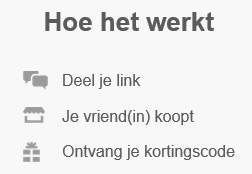
\includegraphics[]{img/hoe-het-werkt.png}
	\centering
	\caption{Hoe het werkt - in drie eenvoudige stappen. Deze boodschap staat onderaan de e-mails in verband met het referral programma.}
	\label{fig:hoe-het-werkt}
\end{figure}

``\emph{Arno} is heel tevreden van Kriket en wil het product aanraden aan zijn vriendin \emph{Bonnie}. Bonnie krijgt volgende URL van Arno opgestuurd via Facebook Messenger ``\emph{https://kriket.refr.cc/arno}``. Bonnie is geïnteresseerd in het concept van Kriket en koopt via de link van Arno een discover box. Door de link van Arno te gebruiken heeft Bonnie 20\% kunnen besparen. Arno krijgt op zijn beurt ook voordeel en ontvangt 20\% korting op zijn volgende aankoop via een kortingscode die hij per mail krijgt opgestuurd.``

De klant maakt kennis met het referral programma via:
\begin{itemize}
	\item E-mail van Kriket naar klanten om de actie aan te kondigen
	\item Post op sociale media met link naar de landingspagina (\href{https://kriket.referralcandy.com}{https://kriket.referralcandy.com})
	\item Pop-up na aankoop in de webshop
	\item E-mail die na aankoop wordt verstuurd
\end{itemize}

Via de pop-up (zie figuur \ref{fig:referral-popup-webshop}) en e-mail krijgt men de link meteen en deze kan dan gedeeld worden. Via de landingspagina moet men natuurlijk eerst een e-mailadres doorgeven zodat de link op basis hiervan aangemaakt kan worden. Het e-mailadres wordt dan gekoppeld met de link en indien een vriend(in) een aankoop doet via deze link wordt de kortingscode hier naar opgestuurd. 

Indien de link werd aangemaakt en gedurende 2 weken niet gebruikt werd, krijgt de klant een vriendelijke herinneringsmail met de boodschap om 20\% korting niet te laten vliegen.

\begin{figure}
	\centering
	\begin{subfigure}{.5\textwidth}
		\centering
		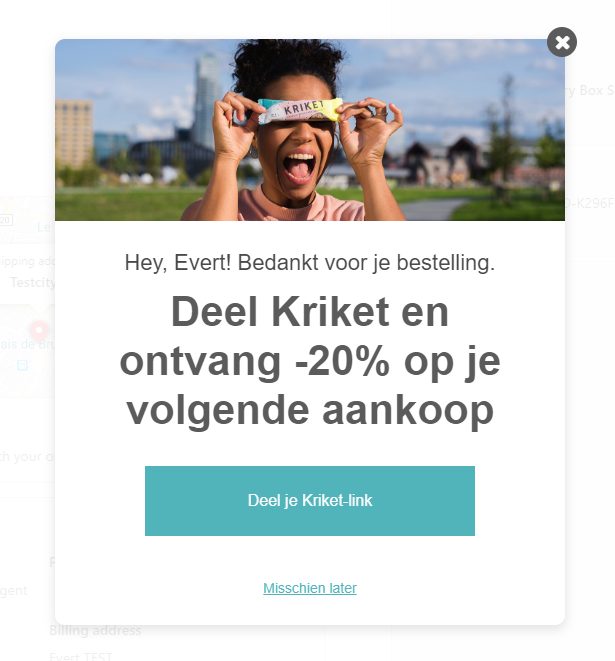
\includegraphics[width=.8\linewidth]{img/referral-pop-up-1.png}
		\caption{Initiële pop-up}
		\label{fig:referral-popup-webshop-1}
	\end{subfigure}%
	\begin{subfigure}{.5\textwidth}
		\centering
		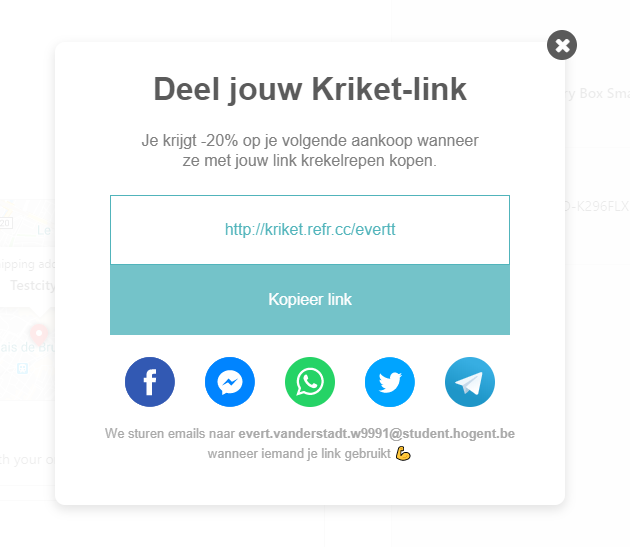
\includegraphics[width=.9\linewidth]{img/referral-pop-up-2.png}
		\caption{Na klik op de knop}
		\label{fig:referral-popup-webshop-2}
	\end{subfigure}
	\caption{Pop-up na aankoop in de Kriket webshop, hieruit kan de link rechtstreeks gekopieerd en gedeeld worden.}
	\label{fig:referral-popup-webshop}
\end{figure}

Zodra de link, \emph{https://kriket.refr.cc/arno}, wordt bezocht, gaat deze je automatisch doorsturen naar een pagina met bijvoorbeeld volgende URL \emph{https://go.referralcandy.com/share/K296FLX} (zie figuur \ref{fig:referral-share-page}). 

Op deze pagina ziet men de kortingscode (ook ``coupon`` genoemd), die 20\% korting geeft op de \emph{Discover Boxes}. Men kan de kortingscode kopiëren door op de tekst te klikken, maar deze wordt ook automatisch toegepast door op de CTA (Call To Action) - ``Bekijk de webshop`` te drukken. Via een aangepaste URL wordt de kortingscode bij het betaalproces automatisch ingevuld. Wanneer deze code gebruikt wordt bij een aankoop krijgt de eigenaar van deze link (en daaraan gekoppeld - de kortingscode), \emph{Arno} in die voorbeeld, een e-mail toegestuurd met een kortingscode voor zichzelf. Met deze code krijgt hij 20\% korting op zijn volgende aankoop.

\begin{figure}[h!]
	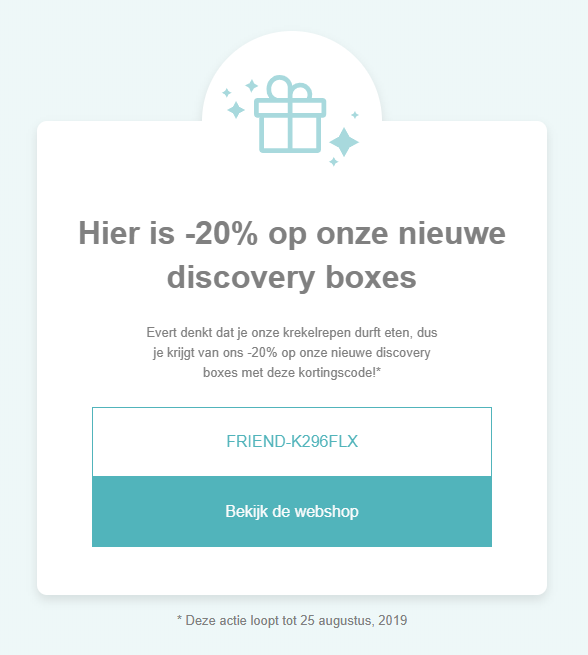
\includegraphics[width=80mm,scale=0.7]{img/referral-share-page.png}
	\centering
	\caption{Deze pagina krijgt de vriend(in) of kennis te zien wanneer de link (bijvoorbeeld \emph{https://kriket.refr.cc/arno}) wordt bezocht.}
	\label{fig:referral-share-page}
\end{figure}

Indien de gebruiker al zijn kortingscodes wil bekijken, kan deze dat doen via de pagina waar hij/zij de link heeft gecreëerd en gekopieerd. Bijvoorbeeld - \emph{https://kriket.referralcandy.com/MWGS976}, wanneer men daar op ``Jouw kortingscodes`` drukt gaat men naar een log-in pagina waar men vervolgens een wachtwoord kan creëren. Hierna kan men de pagina met kortingscodes bekijken - \emph{https://kriket.referralcandy.com/MWGS976/rewards} (zie figuur \ref{fig:referral-account.png}). Men kan hier ook zijn of haar persoonlijke link aanpassen (bijvoorbeeld \emph{https://kriket.refr.cc/evertv})

\begin{figure}[h!]
	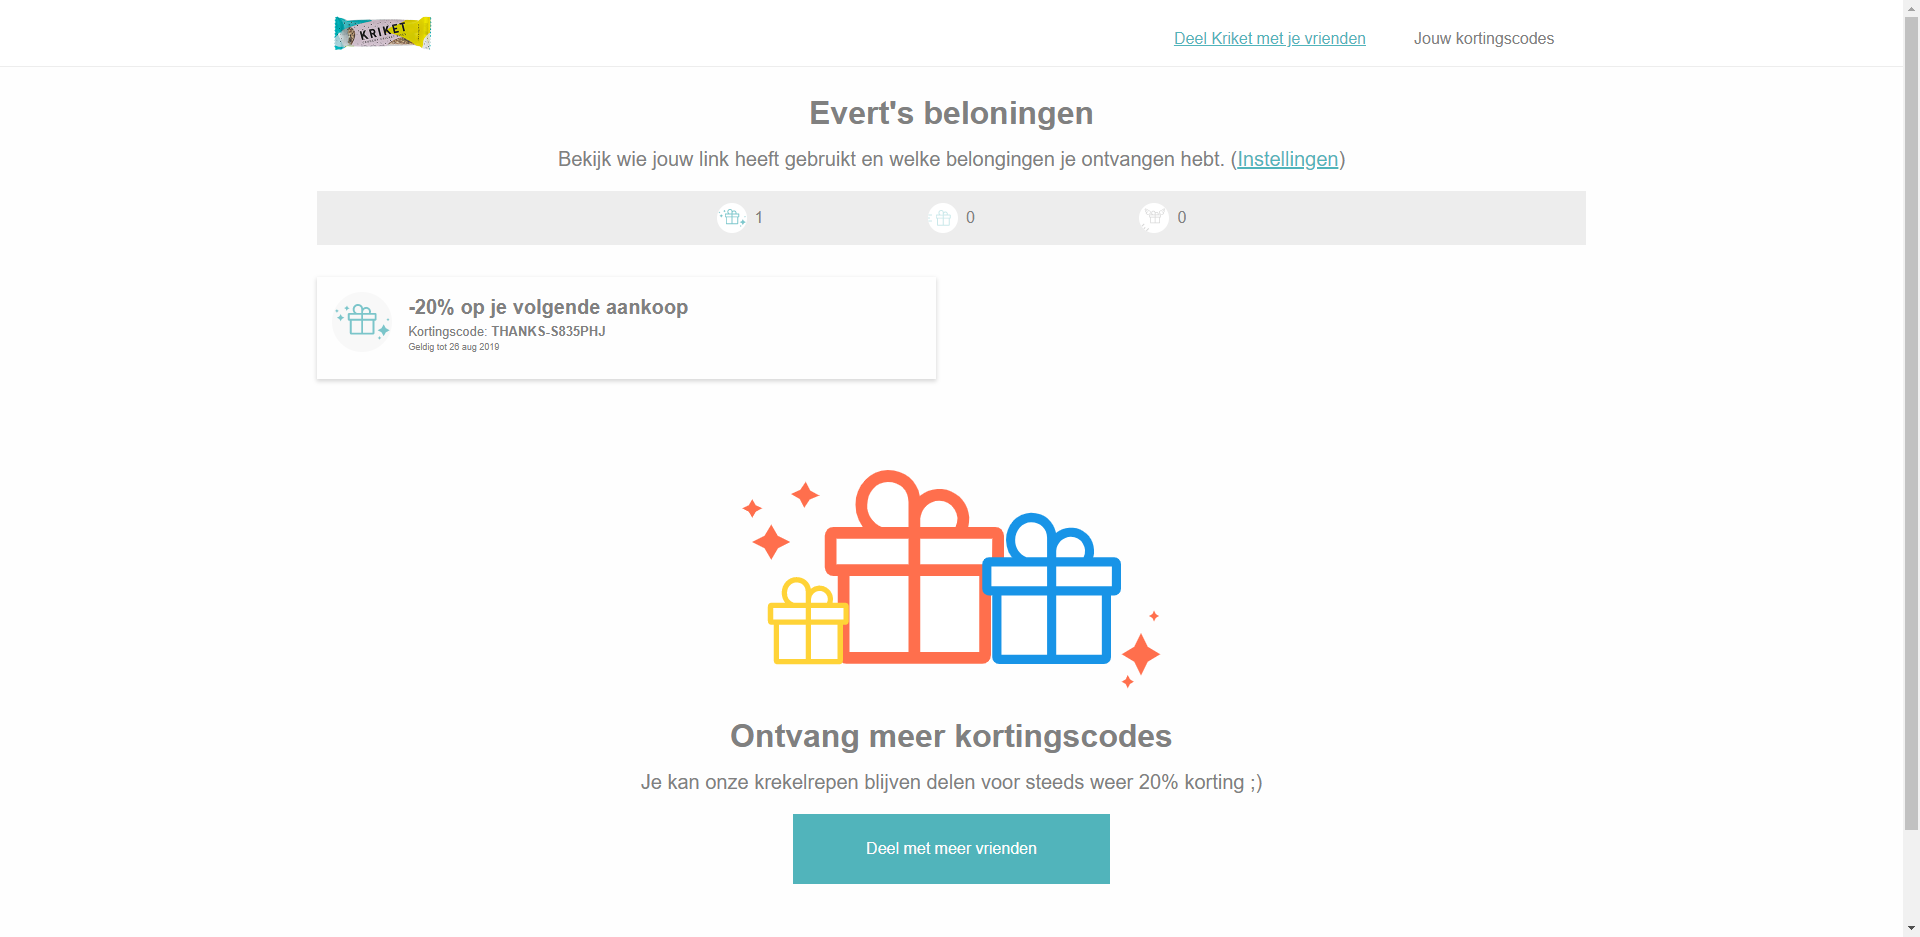
\includegraphics[width=80mm,scale=0.9]{img/referral-account.png}
	\centering
	\caption{Het overzicht van de kortingscodes van een gebruiker.}
	\label{fig:referral-account.png}
\end{figure}

Vanuit Referral Candy is er ook een nieuwe koppeling met Analytics toegevoegd. Een nieuwe \emph{property} werd aangemaakt genaamd ``Referral Program``, een \emph{property} is een onderdeel van een Analytics account. Een property kan een website, mobiele applicatie of dergelijke zijn. In dit geval is Referral Candy onze nieuwe applicatie die we koppelen aan de account. Deze staat dus los van de andere property, ``www.kriket.be``, die de eerder vermelde doelen bevat. Ze ontvangen de data van andere bronnen, de ene van Shopify en de andere van Referral Candy.

Tot slot was een groot deel van het opzetten van Referral Candy om goede tekst te bedenken, copywriting is een vak apart - het marketing gedeelte is daar niet weg te denken. De teksten voor de pop-up, e-mails, landingspagina, overzicht pagina, enzovoort... waren een belangrijk en tijdrovend onderdeel van dit proces. 

\subsection{Discovery box toevoegen} \label{sec:aanpassingen-webshop}
De discovery box wordt in een kleine en grote variant op de webshop geplaatst. Deze producten ``DISCOVERY BOX SMALL`` en ``DISCOVERY BOX LARGE`` worden gebruikt in het referral-programma. De nieuwe klant die de kortingscode van een vriend gebruikt krijgt op deze twee producten 20\% korting. Zo kan men alle krekelrepen uitproberen en zijn of haar favoriet vinden.

\begin{figure}[h!]
	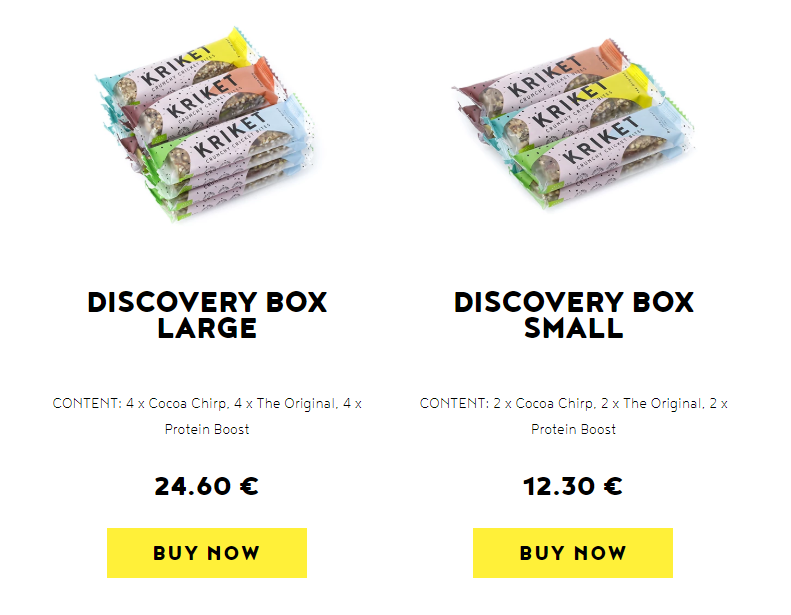
\includegraphics[width=\linewidth]{img/discovery-box-webshop.png}
	\caption{De twee nieuwe producten in de webshop.}
	\label{fig:discovery-box-webshop}
\end{figure}

Naast deze nieuwe producten toe te voegen worden de afbeeldingen verkleind. Het kleiner maken van de afbeeldingen zorgt voor een snellere laadtijd en een aangenamere surf-ervaring op de webshop. Bij sommige producten is het verschil in bestand-grootte enorm, van 800Kb naar 100Kb. Tot wel 8 keer kleiner, het is een opvallend verschil in laadtijd - zeker op een tragere mobiele netwerkverbinding.

\subsection{Growth hack online zetten} \label{sec:growth-hack-online-zetten}
Zodra het opzetten van alle voorgaande tools getest is kan de growth hack online gezet worden. Hierbij worden de twee sociale media platformen gebruikt. Langs Instagram en Facebook komen de fans en klanten van Kriket te weten dat het referral systeem beschikbaar is. 

Initieel wordt via Facebook een post gezet die aankondigt dat de actie van start gaat. Op het einde van de periode wordt er geëxperimenteerd met gesponsorde berichten op Instagram en Facebook. Via deze gerichte advertenties wordt de kans op nieuwe klanten vergroot.

Naast deze sociale media platformen wordt de klant ook op de hoogte gebracht via een pop-up na betaling en via e-mail. Beide ontvangt de klant na het plaatsen van een bestelling, zoals eerder vermeld (zie \ref{sec:referral-candy-toevoegen}). 

\subsection{Monitoring gedurende één maand} \label{sec:monitoring-gedurende-twee-weken}
Tijdens dat de growth hack online staat kan Shopify, Google Analytics en de back-end tool van Referral Candy gebruikt worden voor de monitoring van deze growth hack. Daar kan men opvolgen hoeveel klanten hun link delen via sociale media, wanneer er via iemand zijn of haar link een aankoop is gebeurd, enz...

De growth hack werd gelanceerd op vrijdag 26 juli. Vanaf dat moment kregen de klanten een pop-up en e-mail na betaling in verband met het referral programma. 

De Facebook-post werd geplaatst op woensdag 7 augustus en de gesponsorde posts kwamen hier kort achter. De gesponsorde posts werden in actie gezet nadat de respons op het referral programma klein bleek te zijn. Hierdoor kreeg deze actie meer aandacht en werd het waarschijnlijk meer overwogen door de (potentiële) klanten. Het kan ook een aanzet geven naar mond tot mond reclame, wat anders niet gebeurd zou zijn.

Tijdens de monitoring van 26 dagen werden er geen aanpassingen doorgevoerd aan het referral-programma zelf. Op technisch vlak waren er geen problemen, alle e-mails, kortingscodes, pop-ups en dergelijke werkte zoals gepland.

Tot slot zijn er ook vooraf geen doelen opgesteld, wat in het vorige hoofdstuk \ref{ch:conclusie} wel vermeld werd. Het was in dit geval minder van toepassing omdat het geen iteratief proces is, men laat de growth hack actief lopen voor één maand tijd en analyseert achteraf de data. Indien men deze growth hack een langere periode laat lopen is het interessant om doelen te stellen, waaruit achteraf geleerd kan worden. Deze doelen kunnen dan realistischer worden en zorgen voor een betere inschatting van het bedrijf en de klanten ervan.

\subsection{Data analyseren} \label{sec:data-analyseren}
De data uit Google Analytics, Shopify en Referral Candy capteerde van 26 juli tot 20 augustus volgende (interessante) data:

\textbf{Google Analytics}
\begin{itemize}
	\item Paginaweergaven: 2644	
	\item Sessies: 852 (zie figuur \ref{fig:acquisitie-kanalen})
	\item Gem. sessieduur: 1 min 40 sec
	\item Bezoekers: 660 (zie figuur \ref{fig:sessies-per-apparaat})
		\subitem Desktop: 370
		\subitem Mobile: 270
		\subitem Tablet: 20
	\item Taal:
		\subitem NL: 45,17\%
		\subitem EN: 30,36\%
		\subitem DE: 7,25\%
		\subitem FR: 7,25\%
		\subitem ES: 1,81\%
\end{itemize}
\clearpage
\textbf{Shopify}
\begin{itemize}
	\item Sessies: 102 (93 bezoekers)
		\subitem Desktop: 59
		\subitem Mobile: 39
		\subitem Tablet: 4
	\item Orders voltooid: 23
	\item Totale verkoop: EUR 673,10
	\item Conversie ratio  (zie figuur \ref{fig:conversie-ratio-trechter})
		\subitem Product toegevoegd aan winkelmandje: 36,27\% (35 sessies)
		\subitem Betaling bereikt: 30,39\% (31 sessies)
		\subitem Conversies: 19,61\% (20 sessies)
	\item Populairste item: Discovery Box Large
\end{itemize}
\textbf{Referral Candy}
\begin{itemize}
	\item E-mails verstuurd: 48 
		\subitem Uitnodiging e-mails: 35
		\subitem Herinnering e-mails: 13 
	\item Link clicks: 25
	\item Social media shares: 13
	\item Webshop bezoeken: 16
	\item Aankopen via referral: 5 (zie figuur \ref{fig:directe-referral-verkoop})
	\item Referral omzet: EUR 90,00
\end{itemize}

Ook niet onbelangrijk - de aparte aankondigings-e-mail van Kriket naar hun klanten werd door \textbf{de helft} van de ontvangers gelezen.

\begin{figure}
	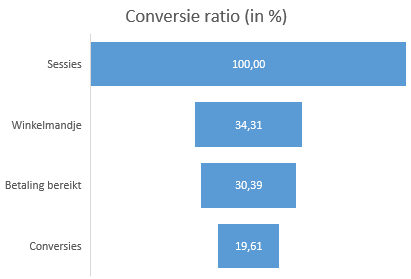
\includegraphics[]{img/conversie-ratio-trechter.png}
	\centering
	\caption{Conversie ratio is 19,61\%, dat wil zeggen dat bijna 1 op 5 sessies eindigt in een aankoop.}
	\label{fig:conversie-ratio-trechter}
\end{figure}

De verkoop data werd enkel uit Shopify gehaald en niet uit Google Analytics. Dit werd gedaan omdat Shopify de data direct bij de bron verkrijgt, Google Analytics kan minder accuraat zijn doordat het in deze situatie werkt met pagina bezoeken. Zo zal Google Analytics kijken naar \emph{/checkout/thank\_you} om te besluiten of er een betaling is gebeurd en Shopify krijgt deze data met 100\% zekerheid binnen omdat deze de betalingen opvolgt. In de tijdsspanne van 26 juli tot 20 augustus heeft Google Analytics 18 voltooide orders getracked en Shopify 23. Vandaar wordt voor deze data Shopify gebruikt.

Het grote verschil in aantal sessies bij Google Analytics en Shopify komt doordat Google Analytics alle sessies van bots mee rekent. Dit kan uitgezet worden bij de instellingen door ``Alle hits van bekende bots en spiders uitsluiten`` aan te vinken. Tijdens deze tests werd dit niet uitgezet en waarschijnlijk is er daardoor een groot verschil. Men kijkt om deze reden voor de beste referentie vooral naar de percentages en de exacte data uit Shopify.

\begin{figure}
	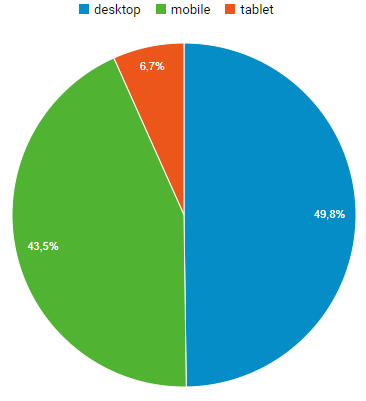
\includegraphics[scale=0.7]{img/sessies-per-apparaat.png}
	\centering
	\caption{Verdeling van aantal sessies op gebruikte apparaten. Men ziet een opvallend groot aantal mobiele gebruikers (43.5\%).}
	\label{fig:sessies-per-apparaat}
\end{figure}
\begin{figure}
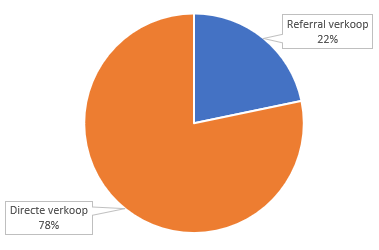
\includegraphics[scale=0.9]{img/directe-referral-verkoop.png}
\centering
\caption{Directe (18 orders) en referral (5 orders) verkoop in een cirkeldiagram.}
\label{fig:directe-referral-verkoop}
\end{figure}
\begin{figure}
	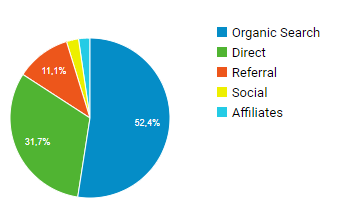
\includegraphics[]{img/acquisitie-kanalen.png}
	\centering
	\caption{De acquisitie kanalen tussen 26 juli en 20 augustus.}
	\label{fig:acquisitie-kanalen}
\end{figure}

Deze data kan men vergelijken met eenzelfde periode, voordat de growth hack in actie werd gezet. Van 1 tot 25 juli, de vergelijking gebeurt best met verkoopcijfers om een duidelijke evolutie te zien voor en tijdens implementatie van  de growth hack. Enkele belangrijke cijfers vindt men in de tabel hieronder.


\begin{tabular}{ |p{4cm}||p{3cm}|p{3cm}|  }
	\hline
	\multicolumn{3}{|c|}{Vergelijking voor en tijdens growth hack} \\
	\hline
	Periode & 1 - 25 juli &26 juli - 20 aug\\
	\hline
	Aantal sessies   & 66    &102\\
	Terugkerende bezoekers   & 42,86\%    &26,09\%\\
	Orders voltooid&   14  & 23\\
	Conversie ratio &21,21\% & 19,61\%\\
	Totale verkoop    &693,40 EUR & 673,10 EUR\\
	Gem. order waarde    &49,53  EUR& 30,81 EUR\\
	\hline
\end{tabular}

Met een gebrek aan toegang tot een databank of .csv-bestand met alle order en bijhorende informatie is het bij bovenstaande gemiddelde niet mogelijk om een standaardafwijking toe te voegen. Deze waarden komen rechtstreeks uit de dashboards van de gebruikte toepassingen.

\subsection{Conclusie: growth hack succesvol?} \label{sec:conclusie-growth-hack-succesvol}
We kunnen uit de laatste tabel hierboven afleiden dat de growth hack vooral voor meer orders heeft gezorgd. Na verder onderzoek zien we een gemiddelde van \textbf{13 à 17 orders per maand} voor de afgelopen maanden. De orders van het referral programma zijn dus bijkomende orders, waardoor het hoogste aantal ooit werd behaald (binnen 26 dagen tijd), \textbf{23 orders}.

Verder is het aantal sessies enorm gestegen, dit is waarschijnlijk mede door de advertenties via Facebook Ads (de sociale media platformen Facebook en Instagram). 

Was de growth hack succesvol? Op het eerste zicht is er niet gigantisch veel veranderd tijdens deze maand, maar het aantal nieuwe bezoekers en nieuwe klanten zorgt waarschijnlijk voor een stabiele groei de volgende maanden. 

De klanten van Kriket zijn mogelijks na 1 maand nog niet genoeg vertrouwd met het referral programma, waardoor ze het nog niet willen gebruiken. Een langere periode zal er voor zorgen dat ze vertrouwd zijn met het systeem. Wanneer ze de nood aan nieuwe krekelrepen voelen, zullen ze denken aan de mogelijkheid om 20\% korting te verkrijgen via dit systeem. Dit heeft waarschijnlijk meer tijd nodig dan een kleine maand. Het is een verhaal dat van enkele klanten ook terug kwam - ze wouden de link doorsturen en kortingscode gebruiken, maar hun kennissen hadden er nog geen nodig of net een order geplaatst. 

Door seizoensgebondenheid en de vakantieperiode wordt er sowieso minder verkocht, vermeld Michiel (medeoprichter van Kriket). Dus dat heeft ook invloed op de cijfers die men tijdens deze periode te zien krijgt.

Verder kan het helpen om enkele influencers, zoals de huidige Kriket Ambassadors \href{https://www.instagram.com/alinefobe}{@alinefobe}, \href{https://www.instagram.com/tiph_duquesne}{@tiph\_duquesne} of \href{https://www.instagram.com/eefdeboeck}{@eefdeboeck}, door een post of Instagramstory\footnote{audiovisuele kortverhalen die 24 uur beschikbaar blijven op de socialenetwerksite} volgers warm te maken voor het referral programma. 

Men ziet op 26 dagen tijd jammer genoeg niet dat Kriket de wereld overneemt met hun krekelrepen. Ondanks dit kan men wel besluiten dat het een succesvolle implementatie was een growth hack op een niet technologische start-up in Brussel. Meer orders, meer bezoekers en (potentiële) klanten hebben Kriket weer eens zien passeren, wat hen mogelijks aanzet om eens krekelrepen te kopen.

Zoals eerder vermeld heeft bijna ieder bedrijf wel een digitale kant in z'n onderneming, via deze weg kan men verschillende growth hacks uitproberen.



